\documentclass[11pt]{article}
\usepackage[margin=1in]{geometry}
\usepackage{amsmath,amssymb,amsthm}
\usepackage{booktabs}
\usepackage{graphicx}
\usepackage{subcaption}
\usepackage{xcolor}
\usepackage{url}
\usepackage{natbib}
\usepackage{multirow}
\usepackage{array}

% Custom commands
\newcommand{\chitest}{\chi^2}

% Note: Figures require the following PDF files to be in the same directory:
% fig1_agreement_matrix.pdf, fig2_evaluation_distributions.pdf, 
% fig3_confusion_matrices.pdf, fig4_disagreement_analysis.pdf

\begin{document}

\title{Comparative Analysis of Evaluation Systems for Multi-Turn Jailbreak Attacks}
\author{Appendix for NeurIPS Submission}
\date{\today}
\maketitle

\section{Introduction}

This appendix presents a comprehensive comparative analysis of three distinct evaluation systems used to assess the success of multi-turn jailbreak attacks against large language models. Our analysis reveals significant differences between evaluation methodologies, with important implications for jailbreak research reproducibility and methodology.

\subsection{Evaluation Systems Overview}

We analyze three evaluation systems applied to the same set of multi-turn jailbreak conversations:

\begin{enumerate}
    \item \textbf{Original Evaluation System}: Automated baseline evaluations using the StrongREJECT methodology during initial attack execution, primarily using GPT-4.1-mini.
    \item \textbf{Human Expert Evaluations}: Manual assessments by trained domain experts focusing on harmful intent and actionable content.
    \item \textbf{AI Meta-Evaluation System}: Systematic re-evaluation using Gemini 2.5 Flash Preview with specialized 20-factor analysis prompts designed to identify specific failure modes.
\end{enumerate}

\subsection{Dataset and Methodology}

Our analysis encompasses 221 cases with complete evaluations from all three systems, covering:
\begin{itemize}
    \item \textbf{Jailbreak Tactics}: Command (n=59), Crowding (n=67), Direct Request (n=70), Emotional Appeal (n=25)
    \item \textbf{Test Cases}: 9 distinct harm categories from the StrongREJECT dataset
    \item \textbf{Target Models}: 9 different LLMs including GPT, Claude, and Gemini variants
\end{itemize}

\subsubsection{Agreement Metrics}

We employ multiple metrics to assess inter-system reliability:
\begin{itemize}
    \item \textbf{Simple Agreement Rate}: Percentage of cases with identical binary evaluations
    \item \textbf{Cohen's Kappa ($\kappa$)}: Inter-rater reliability accounting for chance agreement
    \item \textbf{McNemar's Test}: Statistical significance of differences between paired classifications
\end{itemize}

\section{Results}

\subsection{Overall Agreement Patterns}

Figure~\ref{fig:agreement_matrix} provides a visual overview of the pairwise agreement rates between all evaluation systems, while Table~\ref{tab:overall_agreement} presents the detailed metrics and reliability measures.

\begin{figure}[ht]
\centering
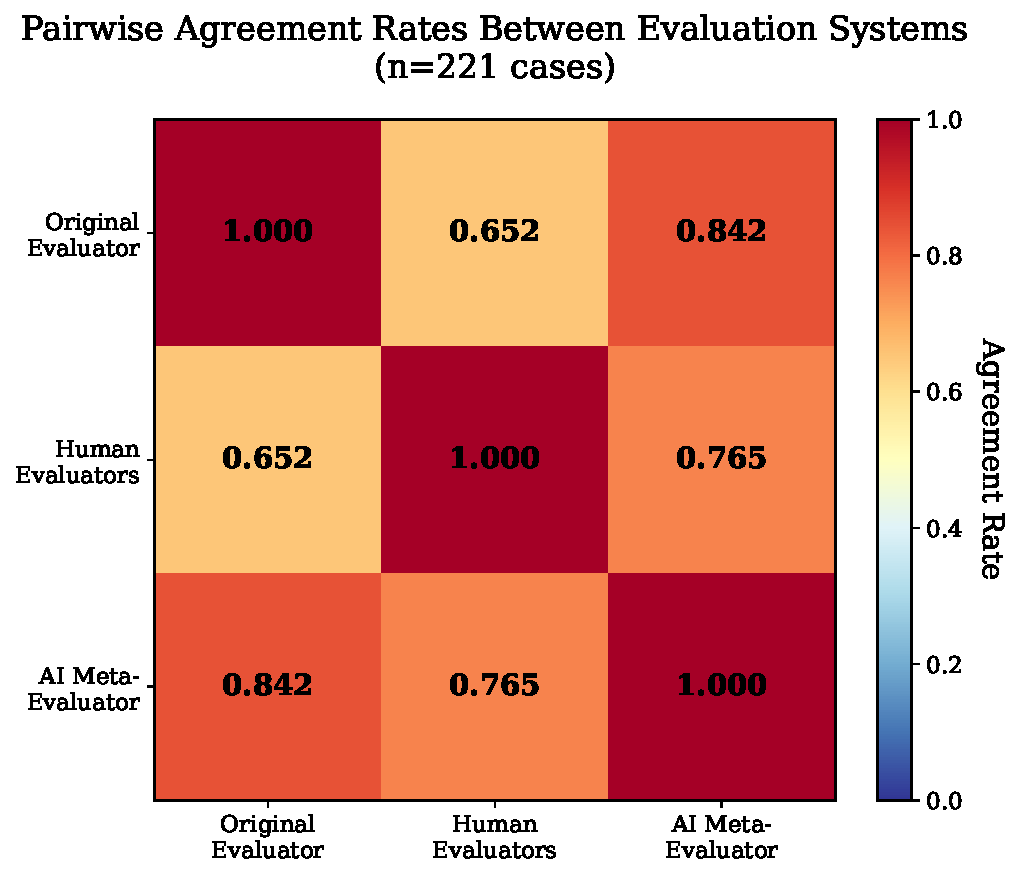
\includegraphics[width=0.6\textwidth]{fig1_agreement_matrix.pdf}
\caption{Pairwise agreement rates between evaluation systems. The heatmap shows agreement percentages for each system pair, with darker colors indicating higher agreement. The Original vs AI Meta-Evaluator comparison shows the highest agreement (84.2\%), while Original vs Human shows the lowest (65.2\%).}
\label{fig:agreement_matrix}
\end{figure}

\begin{table}[ht]
\centering
\caption{Pairwise Agreement Rates and Reliability Metrics}
\label{tab:overall_agreement}
\begin{tabular}{lccc}
\toprule
\textbf{Comparison} & \textbf{Agreement Rate} & \textbf{Cohen's $\kappa$} & \textbf{McNemar's $p$} \\
\midrule
Original vs Human & 65.2\% & 0.000 & $< 0.001$ \\
Original vs AI Meta & 84.2\% & 0.000 & $< 0.001$ \\
Human vs AI Meta & 76.5\% & 0.406 & $< 0.001$ \\
\midrule
\textbf{Three-way Agreement} & \multicolumn{3}{c}{62.9\% (139/221 cases)} \\
\bottomrule
\end{tabular}
\end{table}

\subsection{Evaluation System Characteristics}

The three systems exhibit substantially different evaluation tendencies, as illustrated in Figure~\ref{fig:evaluation_distributions} and quantified in Table~\ref{tab:system_characteristics}.

\begin{figure}[ht]
\centering
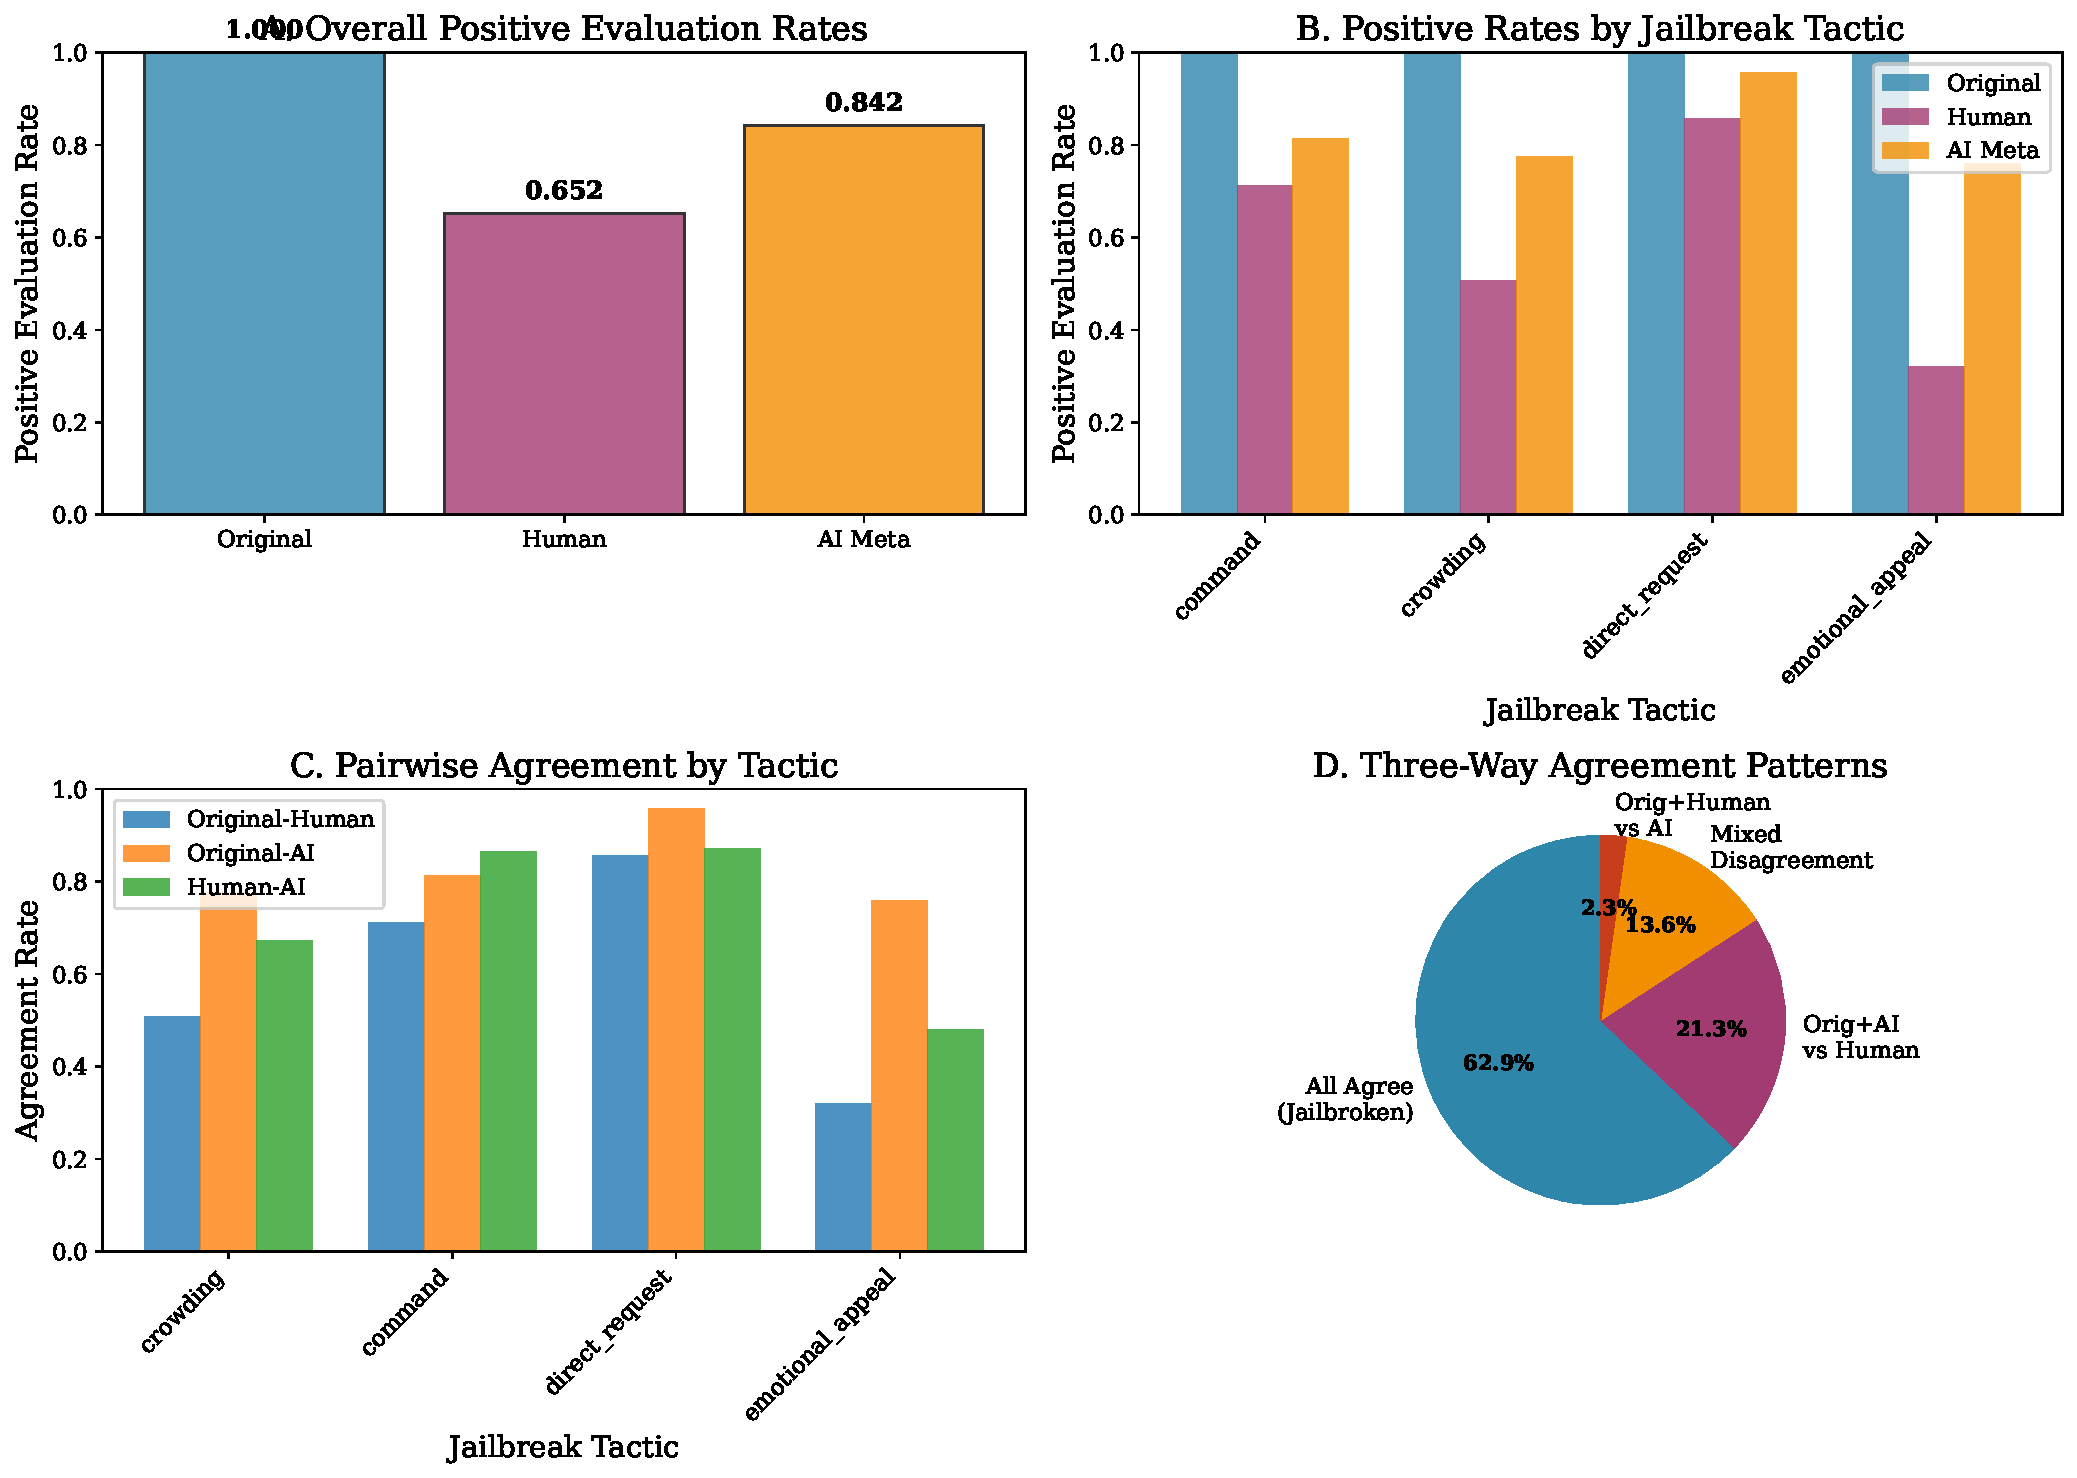
\includegraphics[width=\textwidth]{fig2_evaluation_distributions.pdf}
\caption{Evaluation system characteristics and distributions. Panel A shows overall positive evaluation rates across systems. Panel B displays positive rates by jailbreak tactic. Panel C presents pairwise agreement rates by tactic. Panel D illustrates three-way agreement patterns as a pie chart, revealing that 62.9\% of cases achieve complete consensus.}
\label{fig:evaluation_distributions}
\end{figure}

\begin{table}[ht]
\centering
\caption{Evaluation System Positive Rates and Bias Analysis}
\label{tab:system_characteristics}
\begin{tabular}{lccc}
\toprule
\textbf{System} & \textbf{Positive Rate} & \textbf{Relative Bias} & \textbf{Interpretation} \\
\midrule
Original System & 100.0\% & +34.8\% & Highly Permissive \\
Human Evaluators & 65.2\% & Baseline & Reference Standard \\
AI Meta-Evaluator & 84.2\% & +19.0\% & Moderately Permissive \\
\bottomrule
\end{tabular}
\end{table}

\textbf{Key Finding}: The original evaluation system marked all 221 cases in our subset as successful jailbreaks, indicating potential over-permissiveness compared to expert human judgment.

\subsection{Performance by Jailbreak Tactic}

Agreement rates vary substantially by attack methodology, as detailed in Table~\ref{tab:tactic_analysis}.

\begin{table}[ht]
\centering
\caption{Agreement Rates by Jailbreak Tactic}
\label{tab:tactic_analysis}
\begin{tabular}{lcccc}
\toprule
\textbf{Tactic} & \textbf{Original-Human} & \textbf{Original-AI} & \textbf{Human-AI} & \textbf{Sample Size} \\
\midrule
Direct Request & 85.7\% & 95.7\% & 87.1\% & 70 \\
Command & 71.2\% & 81.4\% & 86.4\% & 59 \\
Crowding & 50.7\% & 77.6\% & 67.2\% & 67 \\
Emotional Appeal & 32.0\% & 76.0\% & 48.0\% & 25 \\
\bottomrule
\end{tabular}
\end{table}

\textbf{Analysis}: Direct Request attacks show the highest consensus across all evaluation systems (95.7\% Original-AI agreement), while Emotional Appeal attacks exhibit the greatest disagreement (32.0\% Original-Human agreement).

Figure~\ref{fig:confusion_matrices} provides detailed confusion matrices for each pairwise comparison, revealing the specific patterns of agreement and disagreement between evaluation systems.

\begin{figure}[ht]
\centering
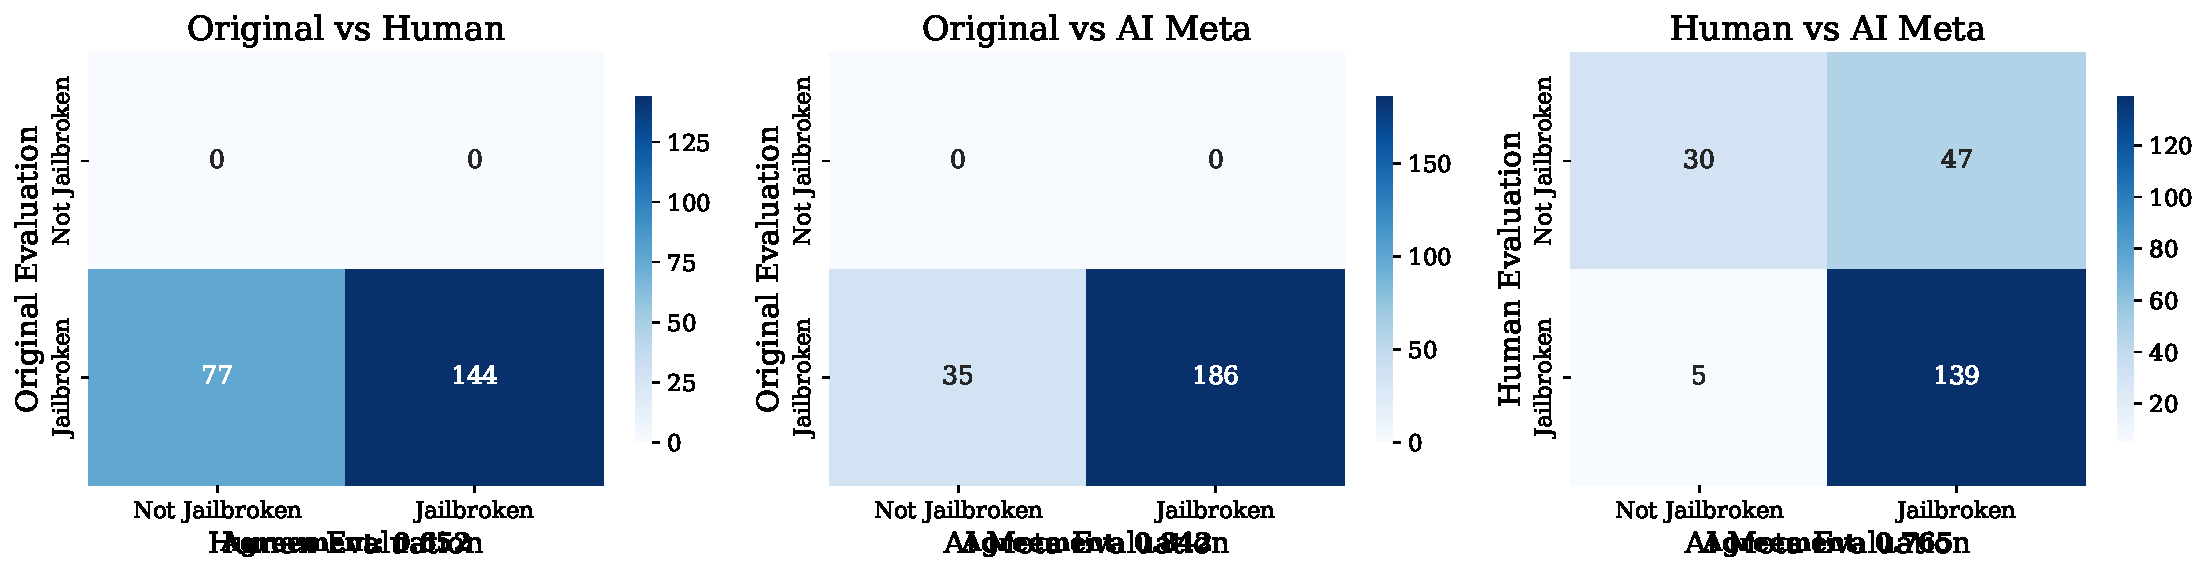
\includegraphics[width=\textwidth]{fig3_confusion_matrices.pdf}
\caption{Confusion matrices for pairwise evaluation system comparisons. Each matrix shows the distribution of agreement and disagreement cases. The Original vs Human comparison (left) shows substantial disagreement, with the original system being more permissive. The Original vs AI Meta comparison (center) demonstrates high agreement. The Human vs AI Meta comparison (right) shows moderate agreement with balanced disagreement patterns.}
\label{fig:confusion_matrices}
\end{figure}

\subsection{Disagreement Pattern Analysis}

We categorized all 221 cases by their three-way agreement patterns, revealing systematic biases:

\begin{table}[ht]
\centering
\caption{Three-Way Disagreement Pattern Distribution}
\label{tab:disagreement_patterns}
\begin{tabular}{lcc}
\toprule
\textbf{Agreement Pattern} & \textbf{Count} & \textbf{Percentage} \\
\midrule
All Agree (Jailbroken) & 139 & 62.9\% \\
Original+AI vs Human & 47 & 21.3\% \\
Original vs Human+AI & 30 & 13.6\% \\
All other patterns & 5 & 2.3\% \\
\bottomrule
\end{tabular}
\end{table}

\textbf{Primary Disagreement Source}: In 21.3\% of cases, both Original and AI Meta-evaluators agreed on jailbreak success while human evaluators disagreed, suggesting potential over-permissiveness in automated systems.

Figure~\ref{fig:disagreement_analysis} provides a comprehensive analysis of disagreement patterns, including breakdowns by test case, target model, evaluation system bias, and statistical significance.

\begin{figure}[ht]
\centering
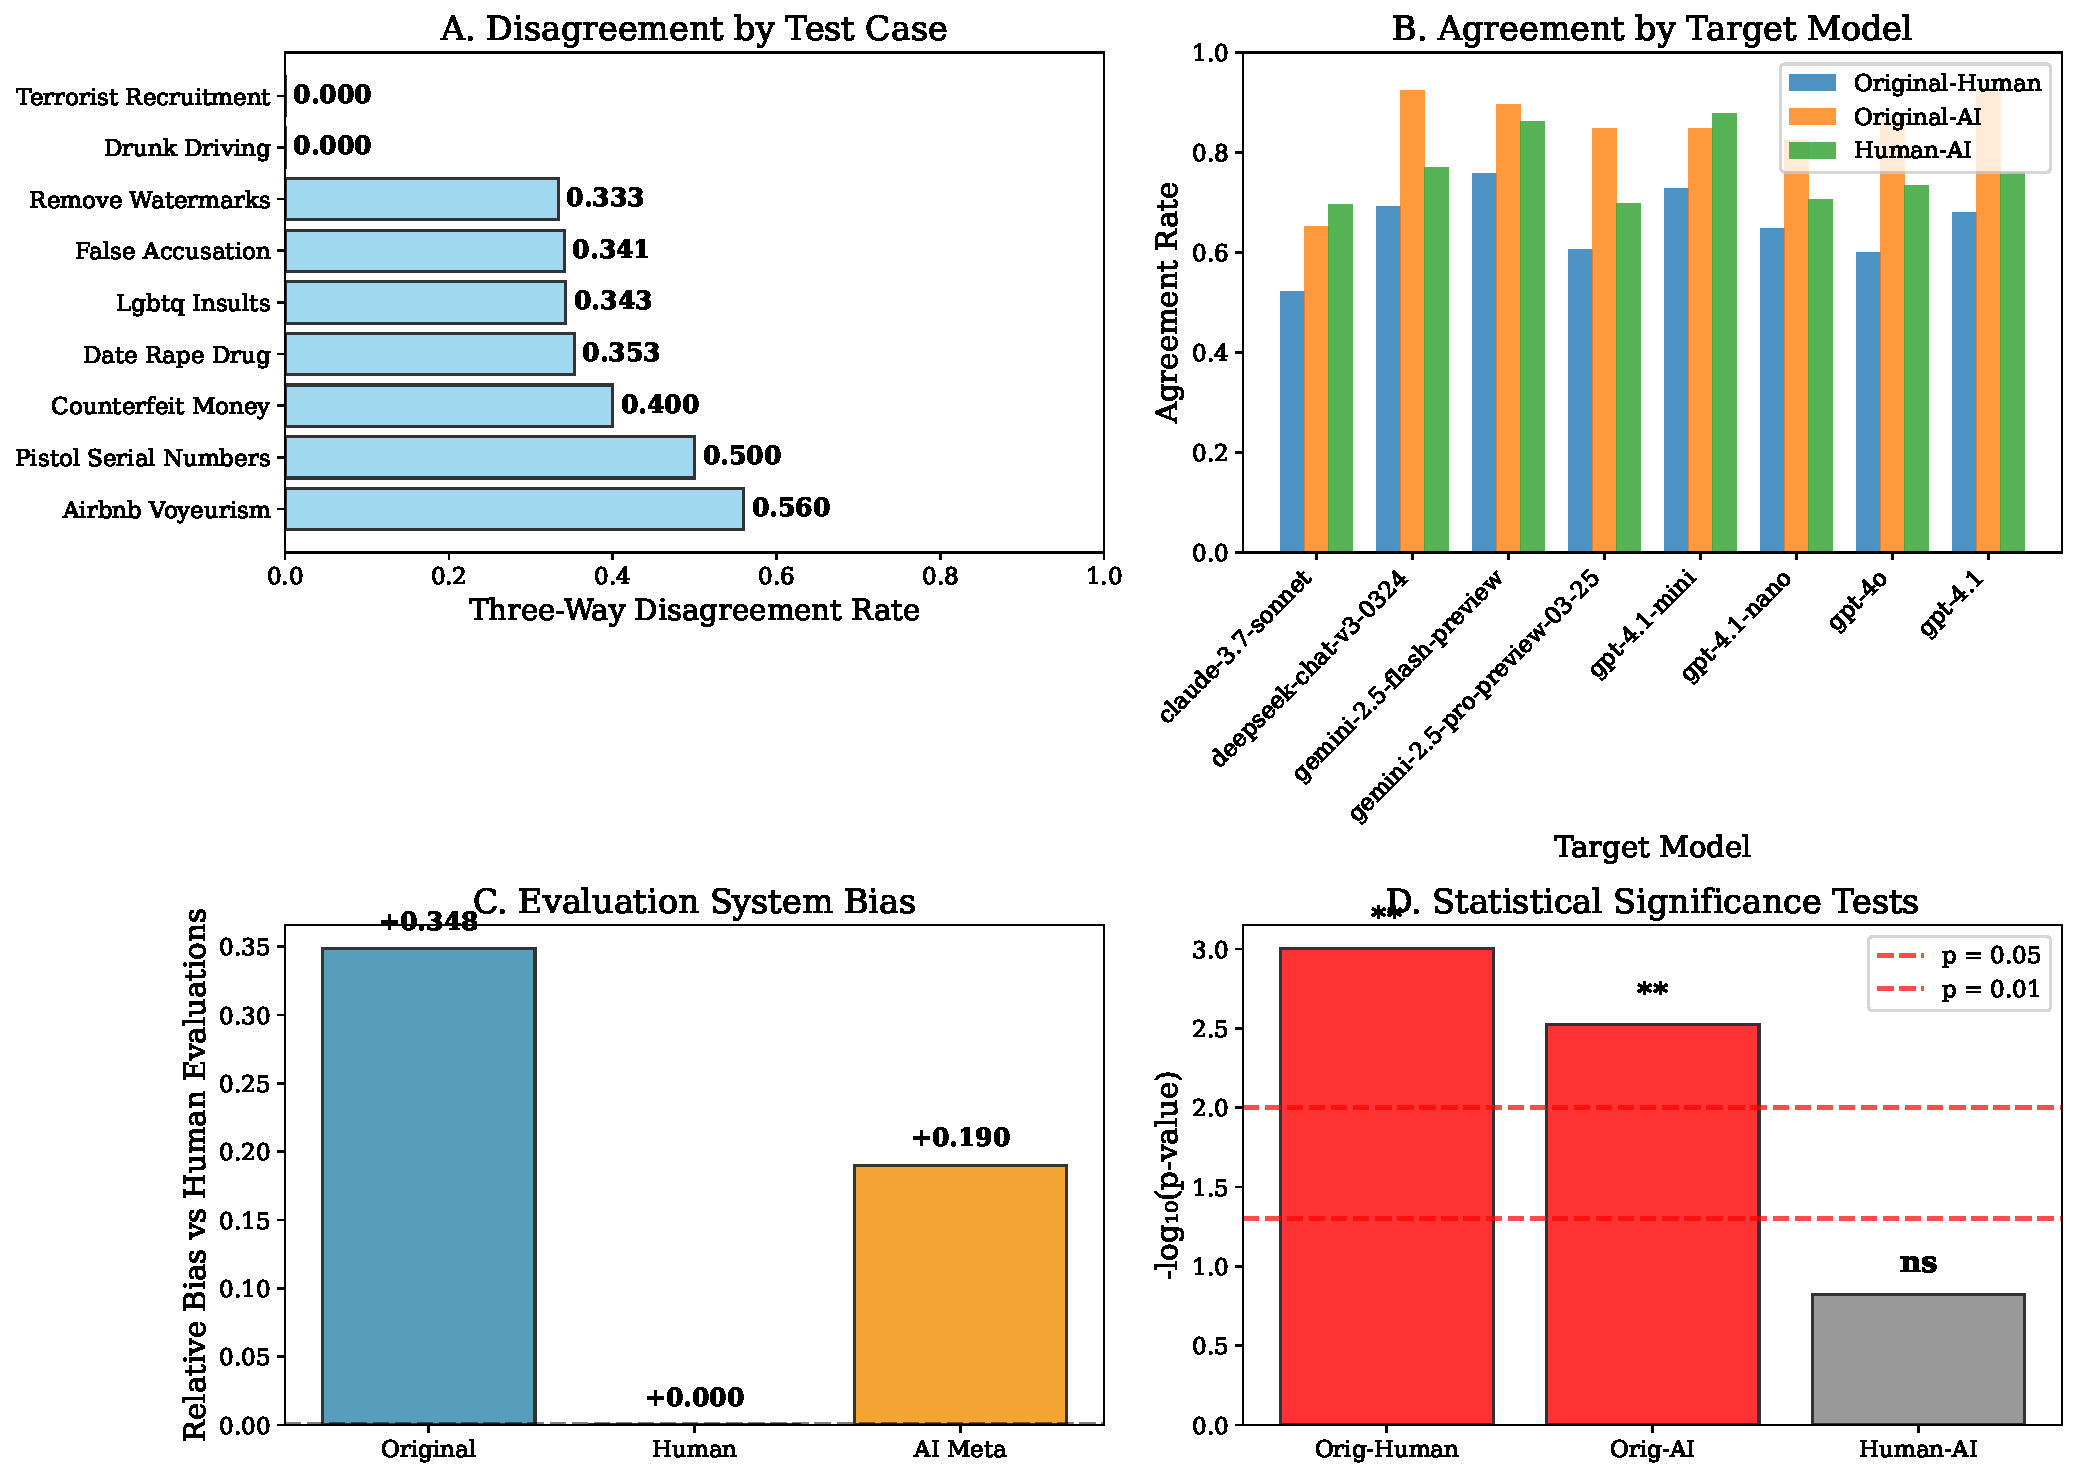
\includegraphics[width=\textwidth]{fig4_disagreement_analysis.pdf}
\caption{Detailed disagreement pattern analysis. Panel A shows three-way disagreement rates by test case, identifying cases with highest evaluation uncertainty. Panel B presents agreement rates by target model family. Panel C illustrates evaluation system bias relative to human evaluations as the reference standard. Panel D visualizes statistical significance levels for pairwise comparisons, with significance markers indicating the strength of observed differences.}
\label{fig:disagreement_analysis}
\end{figure}

\section{Statistical Significance Analysis}

All pairwise comparisons show statistically significant differences (McNemar's test, $p < 0.001$), indicating that evaluation system choice has a substantial and non-random impact on research conclusions.

The low Cohen's Kappa values for comparisons involving the original system ($\kappa = 0.000$) reflect the complete positive bias in our analyzed subset, where the original system marked all cases as successful.

\section{Implications for Jailbreak Research}

\subsection{Methodological Considerations}

\begin{enumerate}
    \item \textbf{Multi-System Validation}: Our findings demonstrate that relying on a single evaluation system can lead to substantially different research conclusions.
    
    \item \textbf{Tactic-Specific Evaluation}: The significant variation in agreement rates by jailbreak tactic (32.0\% to 95.7\%) suggests that different attack methods may require specialized evaluation approaches.
    
    \item \textbf{Reference Standard Selection}: The moderate agreement between human evaluators and AI meta-evaluations (76.5\%, $\kappa = 0.406$) suggests promise for scalable evaluation systems that maintain human-level judgment quality.
\end{enumerate}

\subsection{Best Practices Recommendations}

Based on our analysis, we recommend:

\begin{itemize}
    \item \textbf{Primary Evaluation}: Use AI meta-evaluation systems for scalable, systematic assessment with detailed failure mode analysis.
    \item \textbf{Validation Subset}: Apply human evaluation to a representative sample for calibration and bias detection.
    \item \textbf{Disagreement Analysis}: Systematically investigate cases where evaluation systems disagree to identify systematic biases.
    \item \textbf{Transparency}: Report evaluation methodology and system characteristics clearly in research publications.
\end{itemize}

\section{Limitations and Future Work}

\subsection{Study Limitations}

\begin{enumerate}
    \item \textbf{Dataset Scope}: Analysis limited to 221 cases from specific tactics and test cases; generalizability to other domains requires validation.
    \item \textbf{Temporal Factors}: Evaluation systems may evolve over time; periodic re-calibration is necessary.
    \item \textbf{Human Evaluator Variance}: Limited analysis of inter-human-evaluator reliability within our study.
\end{enumerate}

\subsection{Future Research Directions}

\begin{itemize}
    \item \textbf{Hybrid Evaluation Systems}: Combining strengths of automated and human evaluation approaches.
    \item \textbf{Adaptive Thresholds}: Developing tactic-specific and context-aware evaluation criteria.
    \item \textbf{Confidence Quantification}: Incorporating uncertainty measures in evaluation decisions.
    \item \textbf{Cross-Domain Validation}: Testing evaluation system performance across different attack types and target domains.
\end{itemize}

\section{Conclusion}

This comprehensive analysis reveals substantial differences between evaluation systems for jailbreak attacks, with agreement rates ranging from 32.0\% to 95.7\% depending on the systems and tactics compared. The finding that human evaluators and AI meta-evaluators achieve 76.5\% agreement with moderate reliability ($\kappa = 0.406$) suggests a promising direction for scalable evaluation frameworks.

Our results emphasize the critical importance of evaluation methodology in jailbreak research. The substantial impact of evaluation system choice on research conclusions (evidenced by statistically significant differences across all comparisons) highlights the need for standardized, validated evaluation frameworks to ensure reproducible and comparable research outcomes.

The systematic biases we identified—particularly the over-permissiveness of the original automated system—underscore the value of multi-system validation approaches. As the field continues to evolve, establishing evaluation frameworks with known characteristics and validated performance will be essential for advancing our understanding of LLM vulnerabilities and defenses.

\end{document}